% THIS IS AN EXAMPLE DOCUMENT FOR VLDB 2012
% based on ACM SIGPROC-SP.TEX VERSION 2.7
% Modified by  Gerald Weber <gerald@cs.auckland.ac.nz>
% Removed the requirement to include *bbl file in here. (AhmetSacan, Sep2012)
% Fixed the equation on page 3 to prevent line overflow. (AhmetSacan, Sep2012)

\documentclass{vldb}
\usepackage{graphicx}
\usepackage{balance}  % for  \balance command ON LAST PAGE  (only there!)
\usepackage{algorithm}
\usepackage{algorithmic}
\usepackage{color}

\begin{document}

% ****************** TITLE ****************************************

\title{Speeding Up LSH-Based Similarity Join Through MapReduce Combiner Optimizations}

% possible, but not really needed or used for PVLDB:
%\subtitle{[Extended Abstract]
%\titlenote{A full version of this paper is available as\textit{Author's Guide to Preparing ACM SIG Proceedings Using \LaTeX$2_\epsilon$\ and BibTeX} at \texttt{www.acm.org/eaddress.htm}}}

% ****************** AUTHORS **************************************

% You need the command \numberofauthors to handle the 'placement
% and alignment' of the authors beneath the title.
%
% For aesthetic reasons, we recommend 'three authors at a time'
% i.e. three 'name/affiliation blocks' be placed beneath the title.
%
% NOTE: You are NOT restricted in how many 'rows' of
% "name/affiliations" may appear. We just ask that you restrict
% the number of 'columns' to three.
%
% Because of the available 'opening page real-estate'
% we ask you to refrain from putting more than six authors
% (two rows with three columns) beneath the article title.
% More than six makes the first-page appear very cluttered indeed.
%
% Use the \alignauthor commands to handle the names
% and affiliations for an 'aesthetic maximum' of six authors.
% Add names, affiliations, addresses for
% the seventh etc. author(s) as the argument for the
% \additionalauthors command.
% These 'additional authors' will be output/set for you
% without further effort on your part as the last section in
% the body of your article BEFORE References or any Appendices.

 %  in this sample file, there are a *total*
% of EIGHT authors. SIX appear on the 'first-page' (for formatting
% reasons) and the remaining two appear in the \additionalauthors section.

\numberofauthors{4}
\author{
% You can go ahead and credit any number of authors here,
% e.g. one 'row of three' or two rows (consisting of one row of three
% and a second row of one, two or three).
%
% The command \alignauthor (no curly braces needed) should
% precede each author name, affiliation/snail-mail address and
% e-mail address. Additionally, tag each line of
% affiliation/address with \affaddr, and tag the
% e-mail address with \email.
%
% 1st. author
\alignauthor
Hangyu Li\\
       \affaddr{Department of Computer Science}\\
       \affaddr{City University of Hong Kong}\\
       \affaddr{Kowloon, Hong Kong}\\
       \email{hangyuli3-c@my.cityu.edu.hk}
% 2nd. author
\alignauthor
Sarana Nutanong\\
       \affaddr{Department of Computer Science}\\
       \affaddr{City University of Hong Kong}\\
       \affaddr{Kowloon, Hong Kong}\\
       \email{snutanon@cityu.edu.hk}
% 3rd. author
\alignauthor 
Hong Xu\\
       \affaddr{Department of Computer Science}\\
       \affaddr{City University of Hong Kong}\\
       \affaddr{Kowloon, Hong Kong}\\
       \email{henry.xu@cityu.edu.hk}
\and
% use '\and' if you need 'another row' of author names
% 4th. author
\alignauthor 
Ha For Yu\\
       \affaddr{Department of Computer Science}\\
       \affaddr{City University of Hong Kong}\\
       \affaddr{Kowloon, Hong Kong}\\
       \email{foryuha2-c@my.cityu.edu.hk}
}
% There's nothing stopping you putting the seventh, eighth, etc.
% author on the opening page (as the 'third row') but we ask,
% for aesthetic reasons that you place these 'additional authors'
% in the \additional authors block, viz.

% Just remember to make sure that the TOTAL number of authors
% is the number that will appear on the first page PLUS the
% number that will appear in the \additionalauthors section.


\maketitle

\begin{abstract}
	Approximate similarity join based on locality-sensitive hashing provide good guarantees on reducing computational cost by sacrificing a predictable loss of accuracy. Implementing it using MapReduce further allows it to scale on large high-dimensional datasets. However, it is often the case that the network cost is a bottleneck in distributed processing environment and poses a challenge for achieving faster and more efficient similarity join. In this paper, focusing on C2LSH-based similarity join on MapReduce, we propose two methods to reduce the network cost by improving the utilization of MapReduce combiners. The methods are based on optimized partitioning scheme for LSH buckets using minimum spanning tree and LSH buckets replication with run-time partition selection. Our experiment result shows that our method perform better than the other two method in both data reduction and time saving.
\end{abstract}




\section{Introduction}
Similarity join is of high importance to many applications such as near-duplicate detections and machine learning (k-nearest neighbor and clustering). Among the techniques to speed up similarity join, those based on randomized techniques such as locality-sensitive hashing (LSH) [1] provide good guarantees on reducing computational cost by sacrificing a predictable loss of accuracy [5].
With the data size growing every day in the era of Big Data, scalability has become an important concern. Distributed programming models such as Bulk Synchronous Parallel and MapReduce [9] allow us to improve data processing capability on large datasets by utilizing resources from scalable computing clusters. However, it is often the case that the network cost is a bottleneck in distributed processing environment and poses a challenge for achieving faster and more efficient similarity join.
To address the network bottleneck of distributed similarity join based on C2LSH [6], in this paper, we propose two methods to reduce the network cost by improving the utilization of combiners. The first method is a LSH buckets partitioning scheme based on cutting a minimum spanning tree (MST), which minimizes the weight of each partition. The second method is to include bucket replication into the MST-based partitioning scheme, with run-time bucket selection using spectral clustering [3]. We experiment both methods on a Memcached [10] similarity join program. Our experiment result shows that our method perform better than the other two method in both data reduction and time saving.
	The remaining sections of this paper are organized as follows. Section 2 provides a brief introduction to related techniques, tools and works. Section 3 explains how C2LSH-based similarity join is implemented in a distributed way and gives a detailed definition of the problem scope. In section 4, we present our two methods to reduce the network cost and analyze their cost models. The experimental results are demonstrated in section 5. Finally, we conclude this paper in section 6.

\section{Preliminaries}
In this section, we briefly introduce locality-sensitive hashing and the similarity join problem, and also some tools and techniques used in our work.

\subsection{Locality-Sensitive Hashing}
Locality-sensitive hashing (LSH) is a dimension reduction technique introduced by Indyk and Motwani [1] to solve near neighbor search problem over high-dimensional large datasets. The basic idea of LSH is similar points are more likely to be close together after a projection. Closer projected points are more likely to be good candidates of near neighbors. Therefore, it is required that similar points are hashed to the same bucket with high probability. LSH hash functions aims to maximize the probability of collision of similar points into the same buckets. Such family of hash functions is called (r, cr, P1, P2)-sensitive with the following properties:
Given a distance function \textbf{d}, for positive reals \textbf{r}, \textbf{c}, \textbf{P1}, \textbf{P2}, and \textbf{$P1 > P2$}, \textbf{$c > 1$},\\
If $d(x, y) \leq r \quad then \quad Pr [h(x) = h(y)] \geq P1$\\
If $d(x, y) > cr \quad then \quad Pr [h(x) = h(y)] \leq P2$\\
Locality sensitive hashing [1], [2] is a Monte Carlo method which addresses the dimensionality problem by transforming a proximity search problem into multiple instances of hash table lookups. Using LSH, the similarity join between two datasets Q and X can be solved by multiple constant-time hash table lookups to find similar items in set X for each query point in Q.
The original LSH method is proposed by Indyk et al. [3] for an internal memory dataset in the Hamming space (l1 norm). Gionis et al. [15] then extend this method for external memory. For the Euclidean distance, Datar et al. [9] propose an LSH function based on the p-stable distribution [20] and an approximate nearest neighbor query processing method.
The original LSH method requires a large number of hash functions to guarantee the accuracy of query results. Panigrahy et al. [16] propose an entropy-based LSH method to improve the quality of lookup results using a limited number of hash functions. Specifically, their method randomly chooses a number of nearby points with respect to the query point q and incorporate their neighbors into the result set in order to reduce the number of false negatives. Their analysis shows that the space consumption is nearly linear with respect to the number of data points.
Dong et al. [17] propose a recursive algorithm for accuracy improvement. The algorithm associates each data point x in X with their approximate kNN result set from X, which is equiv- alent to building a graph which describes the kNN relationships between data points in X. Given a query point q, their method first finds a tentative kNN result set using the basic LSH lookup method. The method then traverses the graph in a recursive fashion while incorporating visited nodes into the tentative result set. The algorithm terminates when the tentative result set is stable.
Lv et al. [5] tackle the space consumption problem using a multi-probing method. Instead of combining result sets from multiple similarity lookups [16], [17], the multi-probing method allows each hash code to be associated with multiple hash buckets. Each hash code lookup requires checking multiple buckets which have a high probability of containing the nearest neighbor of a query point. Their analysis shows that the multi-probe LSH method provides an improved performance in terms of space consumption and time complexity in comparison to the entropy- based LSH method.

\subsection{C2LSH}
Collision Counting LSH (C2LSH) [6] is a variant of the LSH technique for solving c-approximate near neighbor search problem. The idea of C2LSH is that by hashing data points with multiple LSH functions into buckets, similar points should collide more than dissimilar points. By setting a collision threshold L, if point x collides with point y under at least L LSH functions, then x is considered a good candidate of being a near neighbor of y.

\subsection{Similarity Join}
Given two sets of records \textbf{P} and \textbf{Q}, distance function d, similarity threshold \textbf{T}, a similarity join operation finds all pairs of \textbf{(x, y)} such that $\textbf{x} \in \textbf{P}$, $\textbf{y} \in \textbf{Q}$ and $\textbf{d(x, y)} \leq \textbf{T}$.
Techniques for speeding up similarity join on large datasets includes candidate pruning and candidate set generation. Approaches using these techniques on different data types and metric spaces have been well studied by previous researchers. However, not all of them scale well to high-dimensional datasets.

\subsection{LSH-based Similarity Join}
Since LSH functions hash similar data points into the same buckets with high probability, LSH can be used for candidate set generation in approximate similarity join, which may have false positives and negatives. Candidate pairs are generated from data points in each hash bucket. As LSH functions project data points to a single dimension, such technique allows approximate similarity join to scale well regardless of the number of dimensions of the datasets, and therefore avoiding the curse of dimensionality. Previous works using LSH in similarity join include:
Chen et al. [4] presented a way to perform similarity joins on massive time sequences in parallel using LSH and MapReduce. Yuen et al. [2] proposed a framework for approximate string similarity join based on MinHash LSH and trie-based index techniques. Xiong et al. [12] introduced Bucket-Pruning-based LSH indexing to prune expensive similarity computation for top-k similarity join in a heterogeneous information network. Wang et al. [8] propsed Personalized LSH implemented using MapReduce with a new banding scheme to allowing tailoring the number of false positives and negatives for satisfying needs of different application scenarios.

% end the environment with {table*}, NOTE not {table}!

\subsection{MapReduce \& Combiners}
In distributed computing, combiners reduce communication overhead by performing message aggregation at the sender side. Combiners can be applied effectively when messages can be summarized using arithmetic operations such as min, max and sum. Take MapReduce [9] as an example, combiners are used to aggregate data by their keys before the shuffle phrase. In MapReduce, data is expressed as key-value pairs, and computation is represented by three functions:\\
	\indent\indent\indent\textbf{Map					$(k1, v1)		\to	list(k2, v2)$}\\
	\indent\indent\indent\textbf{Combine (optional)		$(k2, list(v2))	\to	(k2, v3)$}\\
	\indent\indent\indent\textbf{Reduce				$(k2, list(v3))	\to	(k2, v4)$}
In actual execution, the mappers run on every computation nodes to generate key-value pairs. Shuffle phrase is then run to send the key-value pairs across the network to group pairs with the same key into the same partition. In the reduce phrase, each reducer gets a list of values with the same key and computes a merged value, which may then be fed to another reducer. The combiner is an optional function with the same signature as the reducer. It is run before the shuffle phrase on each node to merge the partial values by key so to reduce the network cost of the shuffle phrase (See figure 1).


\begin{figure}
\centering
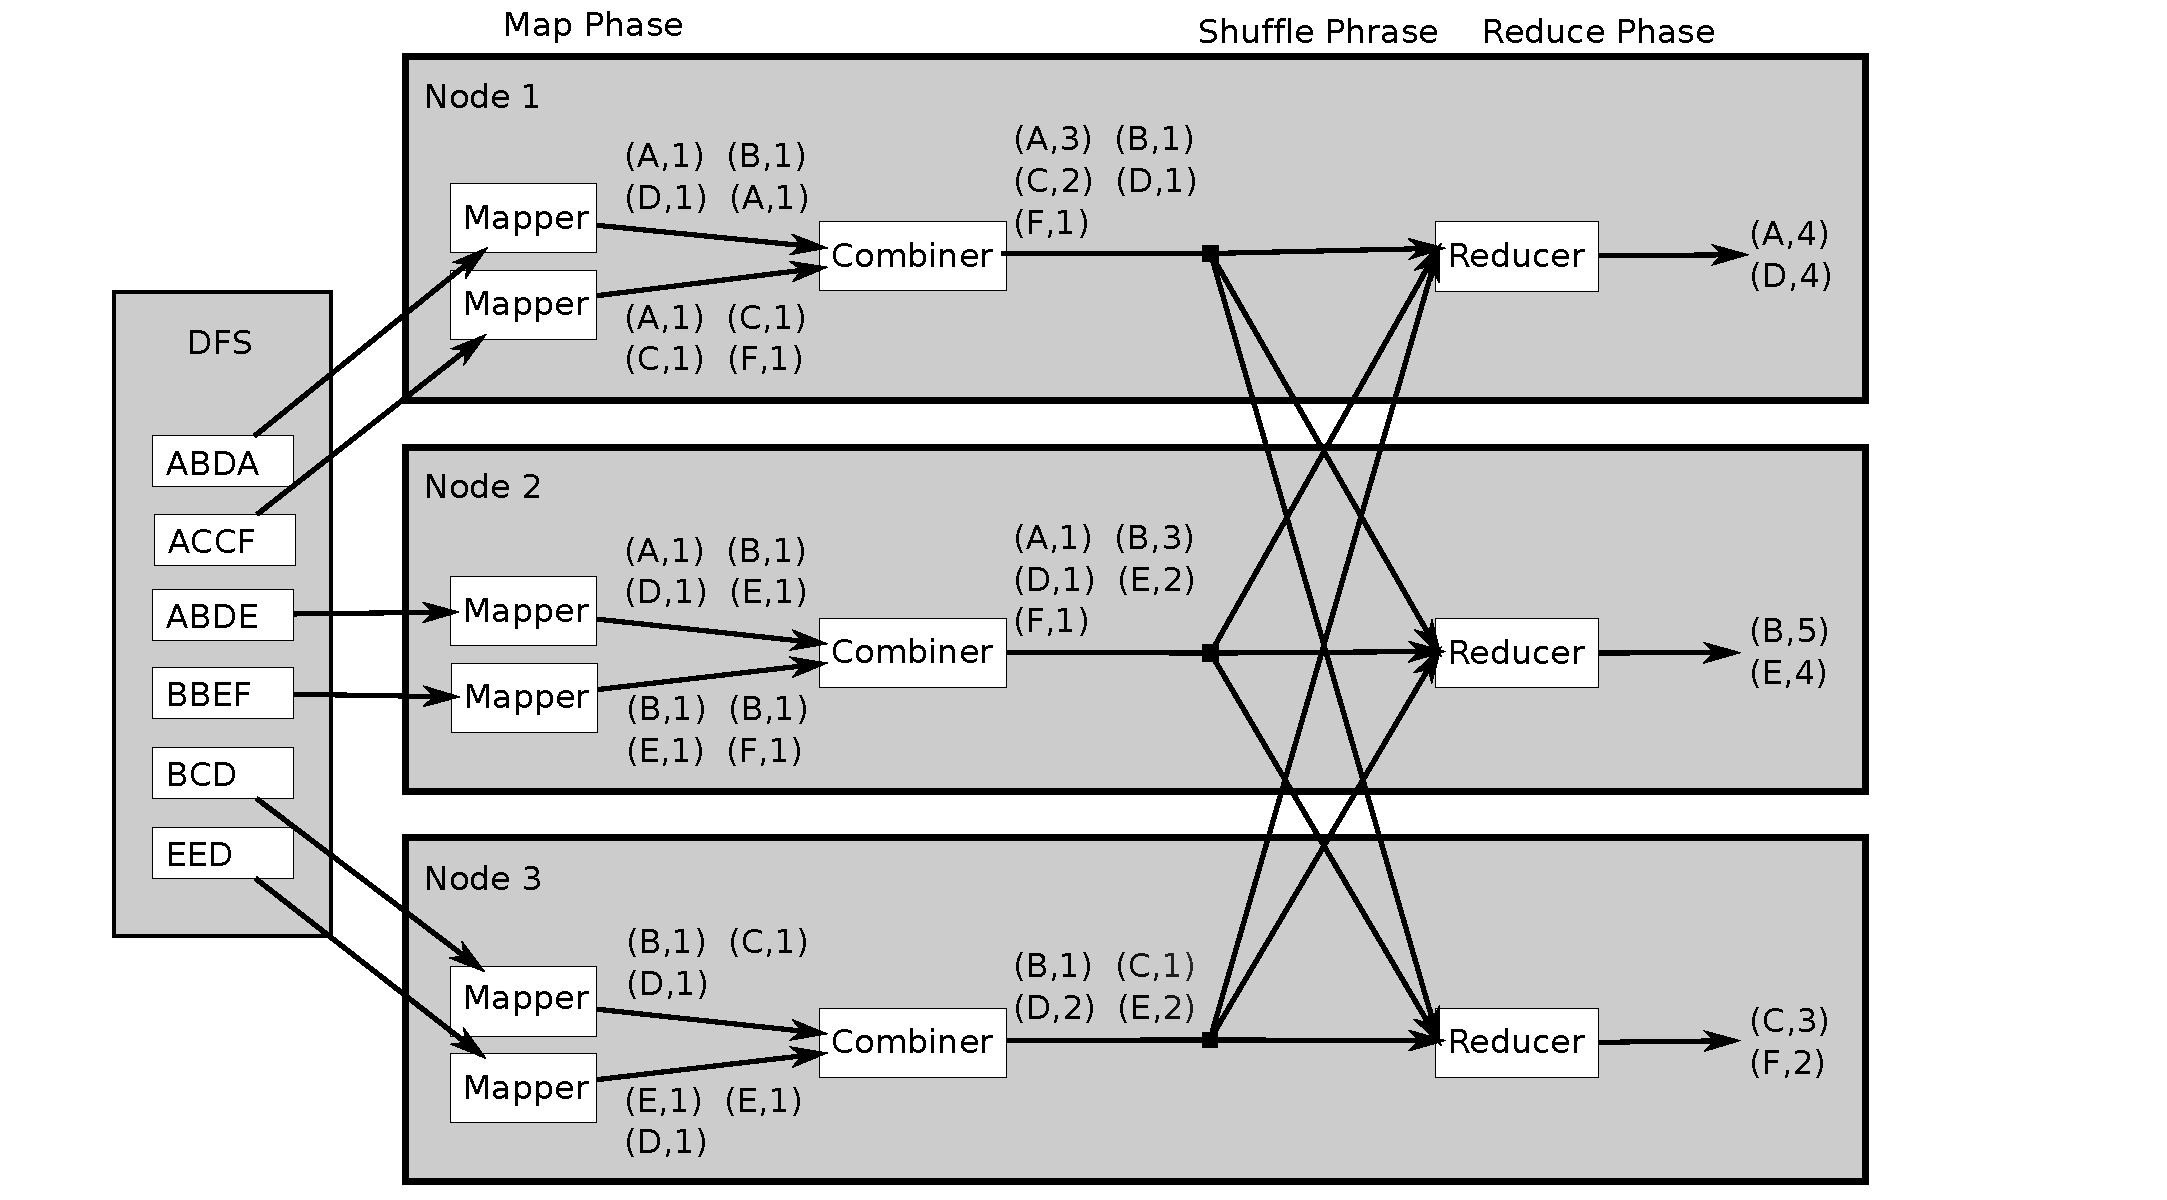
\includegraphics[scale=0.3]{fig1}
\caption{Counting on MapReduce}
\label{fig:fig1}
\end{figure}

\subsection{Memcached}
Memcached [10] is a high performance distributed key-value store. It provides a very large hash table distributed across a cluster. The size of the hash table is limited by the available memory across all the nodes in a cluster. Inserting data into a full Memcached hash table will lead to older data to be purged in least recently used order.

\subsection{Minimum Spanning Tree}
Given a weighted, undirected graph, a minimum spanning tree is a subgraph connecting all the vertices with minimal total weight for the subgraph?s edges. Two famous algorithms for finding minimum spanning tree are Prim's algorithm and Kruskal's algorithm [11].

\subsection{Spectral Clustering}
Spectral clustering [3] is a clustering technique based on graph partitioning. Given a similarity graph and its weighted adjacency matrix representing a dataset, the following steps are performed to map each point to a lower-dimensional representation:\\
1. Form the Laplacian matrix\\
2. Compute the Eigen values and Eigen vectors of the Laplacian matrix.\\
3. Points are represented by vectors extracted from the matrix formed by the Eigen vectors.\\
4. K-means is then performed to cluster the points based on the new representation.

\section{Problem Scope Definition}
In this section, the implementation of C2LSH-based similarity join on MapReduce is explained and the network bottleneck for such implementation is analyzed. Details including problem metric space and the type of LSH functions used in our work are also defined.

\subsection{C2LSH on MapReduce}
In C2LSH, each data point is hashed into multiple buckets using multiple hash functions. Given \textbf{h} hash functions and \textbf{b} buckets per hash function, \textbf{hb} buckets are obtained after hashing. To perform approximate similarity joins between dataset \textbf{P} and \textbf{Q} using C2LSH in distributed environment, data points from both datasets are hashed to the hb buckets, and the buckets are distributed across a cluster.
Since the idea of C2LSH is similar points should collide more than dissimilar points on the number of hash functions, to find out the similar pairs, the collision counts for every possible pairs of $(x, y) \mid x \in P, y \in Q$ are required. To do that on MapReduce, key-value pairs are generated in the Map phrase by doing a Cartesian product between points from \textbf{P} and \textbf{Q} for each bucket, with the keys being tuples of \textbf{(x, y)} and values being integers 1. The key-value pairs are then combined on each node to reduce the number of key-value pairs to be sent across the network. The combined key-value pairs are then grouped by keys in the shuffle phrase and followed by the reduce phrase to calculate the collision counts by key. The similar pairs can then be found by filtering \textbf{(x, y)} with collision counts above a threshold.
The network cost is induced during the shuffle phrase, in which a large amount of key-value pairs has to be sent across the network due to the Cartesian product in the Map phrase. To speed up the join operation, we can group similar buckets on the same node so to increase the probability that more key-value pairs can be combined and the expensive network cost can be reduced. The problem here is to optimize the LSH buckets allocation in the cluster such that the utilization of the combiners can be maximized without degrading the join performance. In this paper, we measure the utilization of the combiners using the combine ratio, which is equal to the number of key-value pairs before combining divided by the number of key-value pairs after combining.

\subsection{Metric Space}
In the paper, we focus on data points in the Euclidean space. After the data points are hashed into the LSH buckets, the similarities between the buckets need to be calculated for bucket allocation optimization. Each bucket is a set of data points and the similarity of a pair of buckets A and B is given by the Jaccard index:

\textbf{J(A, B) = $\frac{|A \cap B|}{|A \cup B|} $}

The Jaccard distance d(A, B) is defined as 1 - J(A, B). With the Jaccard distance calculated for every possible pairs of buckets, we can then represent the buckets as an undirected connected graph, with the buckets being the vertices and the Jaccard distance being the weight of an edge connecting two vertices.

\subsection{LSH based on p-Stable Distribution}
A family H of LSH functions, proposed by Datar et al. [7] for the Euclidean distance, takes the following form:\\
\indent\indent\indent\indent\indent\indent$h_{a,b}(\nu) = \lfloor \frac{a\centerdot\nu+b}{W}\rfloor$\\
a is a vector having the same number of dimension as the data point v, with each entry in a randomly chosen from a p-stable distribution, such as Gaussian distribution N(0,1). b is a real number randomly chosen from the range [0, W]. W is a real number representing the bucket width. In this paper, we use a LSH family G constructed by concatenating k randomly chosen hash functions from H:\\
\indent\indent\indent\indent\indent\indent$g(v) = ( h_{a1,B1}(v),\dots,h_{ak,Bk}(v))$\\
This reduces the probability of having false positives.


\section{MapReduce Combiner Optimizations}
We propose two methods to improve the utilization of the combiners. The first method group similar buckets into the same partition by using a partitioning scheme based on cutting a minimum spanning tree (MST). The second method replicates the buckets partitioned by the first method into other partitions, and uses spectral clustering to select nodes for similarity join at run-time.

\subsection{Partitioning based on Cutting Minimum Spanning Tree}
As mentioned in section 3.2, the buckets can be represented as an undirected, connected graph with the bucket distances as the weights of the edges. By finding a MST of the graph, we can obtain the edges required to build the subtrees which build the MST, and also the order of the last few edges added to connect the subtrees. A property of MST is that the subtrees formed during the MST growing process are also MSTs. These subtrees are partitions of buckets, and their MST properties ensure that each partition has the minimum total weight. Given a cluster of p nodes, the partition assignment for the buckets can be obtained by removing the last p ? 1 edges added to the MST. This gives us p partitions of buckets with the bucket similarity of each partition maximized, and thus increases the probability that the required buckets with high similarity will stay on the same node during a join.
	In actual implementation, the MST partitioning is done in the precomputation so that the same bucket allocation can be used for speeding up multiple joins. However, this also gives us a limitation: The partitioning scheme is independent of the required buckets at run-time. It does not ensure that the combine ratio is maximized for individual query dataset. In other words, this method does not maximize the combine ratio dynamically by using the available information during a join.

\subsection{Bucket Replication with Run-time Partition Selection}
To solve the limitation mentioned in 4.1, we propose to replicate the buckets in each partition after the MST-based partitioning, and the bucket replicas are randomly assign to the other partitions. This introduces the lost randomness back to the bucket allocation so further optimization can be done dynamically based on the required buckets during a join. To illustrate our idea, we provide here a toy example of 10 buckets. Figure 2 shows the distance of the 10 buckets.

\begin{figure}
\centering
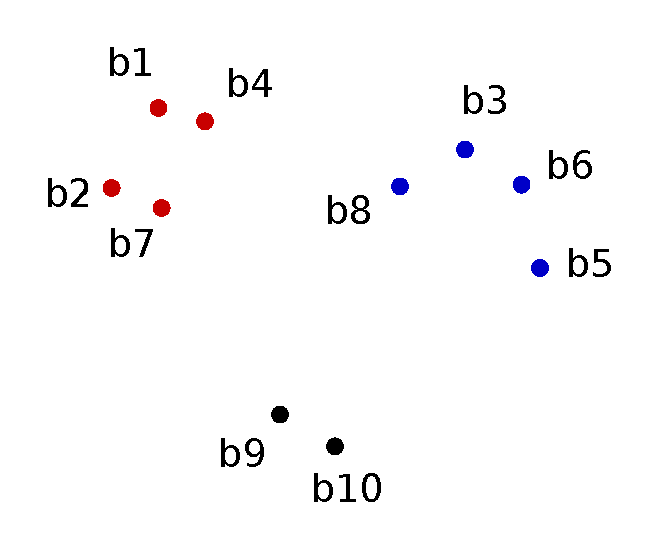
\includegraphics[scale=0.5]{fig2}
\caption{Distance of buckets in a 10-bucket example}
\label{fig:fig2}
\end{figure}

From figure 2, we can see 3 clusters of bucket points. Ideally we would want the bucket allocation to be same as the cluster assignment so to achieve the maximum average combine ratio. However, depending on the number of partitions used, the ideal case may not be achieved. Given a 5-node cluster, we may get the following bucket allocation when using MST-based partitioning:

\begin{table}
\begin{tabular}{|l|l|l|l|}
\hline
\multicolumn{2}{|c|}{IdealCase} &
\multicolumn{2}{c|}{MST-based partitioning}\\
\hline
Node1 & b1,b2,b4,b7 & Node1 & b1,b4\\
\hline
Node2 & b3,b5,b6,b8 & Node2 & b2,b7\\
\hline
Node3 &  & Node3 & b5\\
\hline
Node4 &  & Node4 & b3,b6,b8\\
\hline
Node5 & b9,b10 & Node5 & b9,b10\\
\hline
\end{tabular}
\center
\caption{Bucket allocation without replication}
\center
\end{table}

If a query is performed and the required buckets are b1, b2, b6, b8 and b9, then we can see that the combine ratio is not maximized due to b1 and b2 not staying on the same node. By introducing bucket replication with a replication factor of 3, we may then get the following bucket allocation:

\begin{table}
\begin{tabular}{|l|l|}
\hline
Node1 & \textcolor{red}{b1,b2,b4,b7,}\textcolor{blue}{b8,}b9\\
\hline
Node2 & \textcolor{red}{b1,b2,b7,}\textcolor{blue}{b3,b5,}b9\\
\hline
Node3 & \textcolor{red}{b4,b7,}\textcolor{blue}{b3,b5,b6,}b10\\
\hline
Node4 & \textcolor{red}{b1,b4,}\textcolor{blue}{b3,b6,b8,}b10\\
\hline
Node5 & \textcolor{red}{b2,}\textcolor{blue}{b5,b6,b8,}b9,b10\\
\hline
\end{tabular}
\center
\caption{MST-based partitioning with bucket replication (factor: 3)}
\center
\end{table}

Each node has a larger set of buckets after the replication. This increases the probability that a node may contain a larger subset of the required bucket set of a query. Assume in a query all 10 buckets are required, after the replication we would want to find 3 nodes which have the same bucket subsets as the ideal case in table 1. In table 2, we can see that only node 1 and 5 match with the ideal case. There is no node with all b3, b5, b6, b8 buckets. Therefore, to maximize the combine ratio for this bucket allocation, we have to select a node with the closest possible bucket sets. Given b1, b2, b4, b7 from node 1 and b9, b10 from node 5 are selected, this leaves us with only 5 possible choices:\\

\indent\indent \textbf{Choice 1:}	Node 3 with b3, b5, b6		\textbf{Remaining:}	b8 on Node 1\\
\indent\indent \textbf{Choice 2:}	Node 3 with b3, b5, b6		\textbf{Remaining:}	b8 on Node 5\\
\indent\indent \textbf{Choice 3:}	Node 4 with b3, b6, b8		\textbf{Remaining:}	b5 on Node 2/3\\
\indent\indent \textbf{Choice 4:}	Node 4 with b3, b6, b8		\textbf{Remaining:}	b5 on Node 5\\
\indent\indent \textbf{Choice 5:}	Node 5 with b5, b6, b8		\textbf{Remaining:}	b3 on Node 2/3/4\\

As the goal is to maximize the combine ratio, the distance between the remaining buckets and the selected buckets of other clusters staying on the same node also needs to be considered. For choice 3 and 5, the remaining buckets are not staying with other selected buckets on the same nodes. They are not considered as there is nothing to combine. For choice 1, 2 and 4, the distance between the remaining buckets and the centers of the clusters on the same node are calculated. Only the one with the minimum cost are selected (See figure 3).

\begin{figure}
\centering
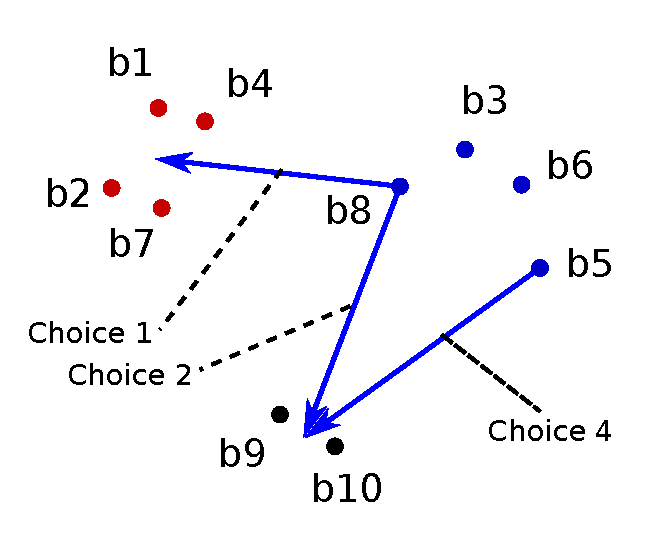
\includegraphics[scale=0.5]{fig3}
\caption{Measure cost for remaining buckets}
\label{fig:fig3}
\end{figure}

Since choice 1 attains the minimum cost, the final selected buckets are b1, b2, b4, b7 ,b8 from node 1, b3, b5, b6 from node 3, and b9, b10 from node 5.
	To perform the above bucket selection process, clustering result needs to be calculated for the required buckets at run-time. We propose to perform spectral clustering on the required bucket set. In general, the bucket selection process is shown as follow in figure 4.
	
\begin{algorithm}
\caption{Node selection}
\label{alg:A}
\begin{algorithmic}[1]
\REQUIRE Spectral Clustering Result C,NodeList N
\FOR {$cluster \in C$}
\FOR {$node \in N$}
\IF {$cluster \in node$}
\STATE add cluster to PrefectMatchList
\ELSE
\IF {node contains most bucket of cluster}
\STATE add to the PrefectMatchList
\STATE assign the remain bucket to the second close cluster c1 
\STATE update the new cluster and add it to the PrefectMatchList
\ENDIF
\ENDIF
\ENDFOR
\ENDFOR
\RETURN {PrefectMatchList}
\end{algorithmic}
\end{algorithm}

\begin{figure}
\centering
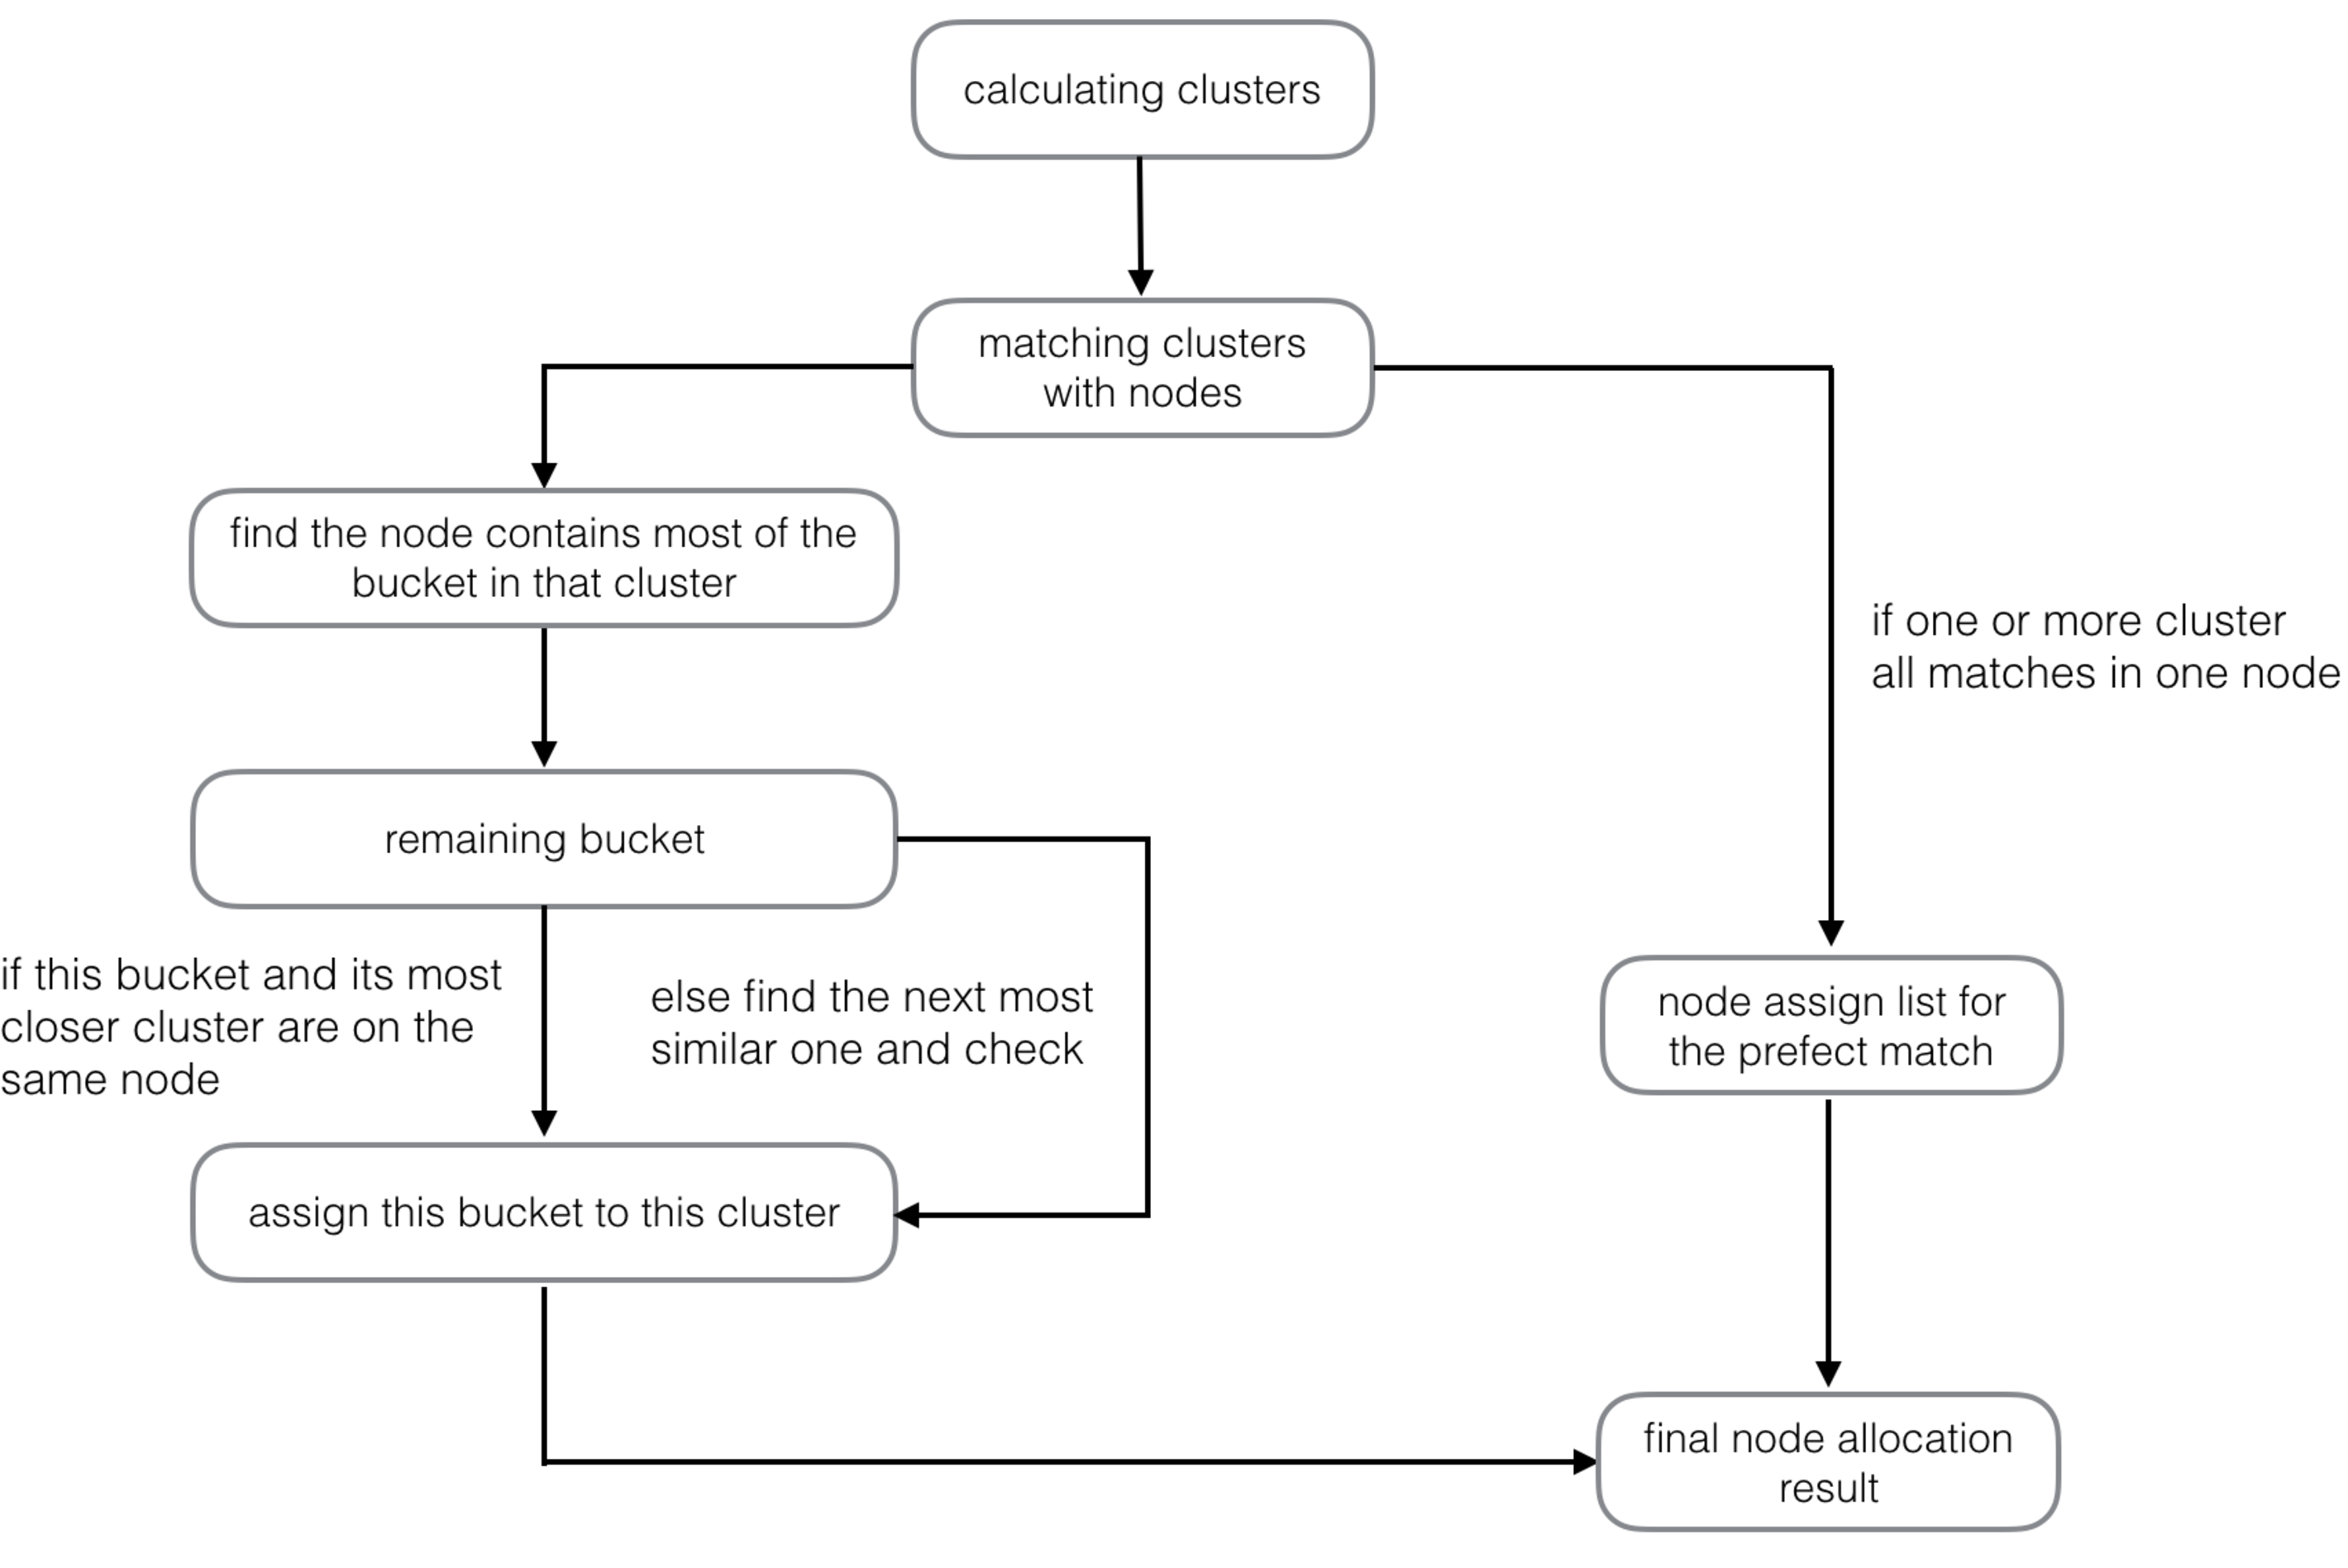
\includegraphics[scale=0.18]{fig4}
\caption{General steps for node selection}
\label{fig:fig4}
\end{figure}
	Since clustering is an expensive operation, in actual implementation some precomputation can be done, and the precomputation result can be used to speed up the run-time clustering process. In the precomputation stage we have calculated the similarity matrix between all the buckets and use the similarity to do the MST bucket allocation. In the bucket selection stage. We use spectral clustering to do the clustering and we also need the similarity as the input. So if we reuse the similarity matrix generated in the precomputation stage we can save the time of calculating similarity again.
\subsection{Predicting the Combine Ratio}
Given L hash functions, B buckets per hash functions, N nodes in a computing cluster, and R replications for each bucket, the approximation of the combine ratio can be calculated as follows:
Before bucket replication, for each of the L hash function, a point pair \textbf{x} can only show on one particular hash function once.There are L hash functions. So this pair can appear in L buckets. Therefore, there are L buckets containing same point pair \textbf{x}  and the probability  that two of these L buckets with point pair \textbf{x}  existing on the same node is close to  given LB buckets are MST-partitioned and $B \ll N$. We assume MST have a probability \textbf{p\%} to assign the similar bucket to a particular node. So that particular node will contain \textbf{L*p\%} similarity buckets. So there are \textbf{L*(1-p\%)} spread in the other \textbf{N - 1} nodes. Let us assume that these buckets are randomly spread into the rest of the nodes. The probability of all these buckets allocated in one node is \textbf{$p_{1}$} , allocated in two node's probability is \textbf{$p_{2}$} ....... all these buckets allocated in all (N-1) node's probability is \textbf{$p_{N-1}$}, So the expectation of the output for N-1 other nodes $Ex_{other}$=$\frac{\sum_{i=1}^{N-1}p_{i}}{N-1}$, the output of \textbf{L*p\%} will always be one. So the final output expectation $Ex = 1 + Ex_{other}$. As we can see on the equation. If we increase p\%, more similar buckets will be assigned to one node and their output will still be 1, but because \textbf{L*(1-p\%)} decreased so $Ex_{other}$ will decrease. So the total output expectation will decrease. Finally we get a lower output.\\
After bucket replication, R - 1 replica for each bucket are randomly assigned to other nodes. The probability that 2 buckets with point x existing on the same node is also increased. .

\begin{figure}
\centering
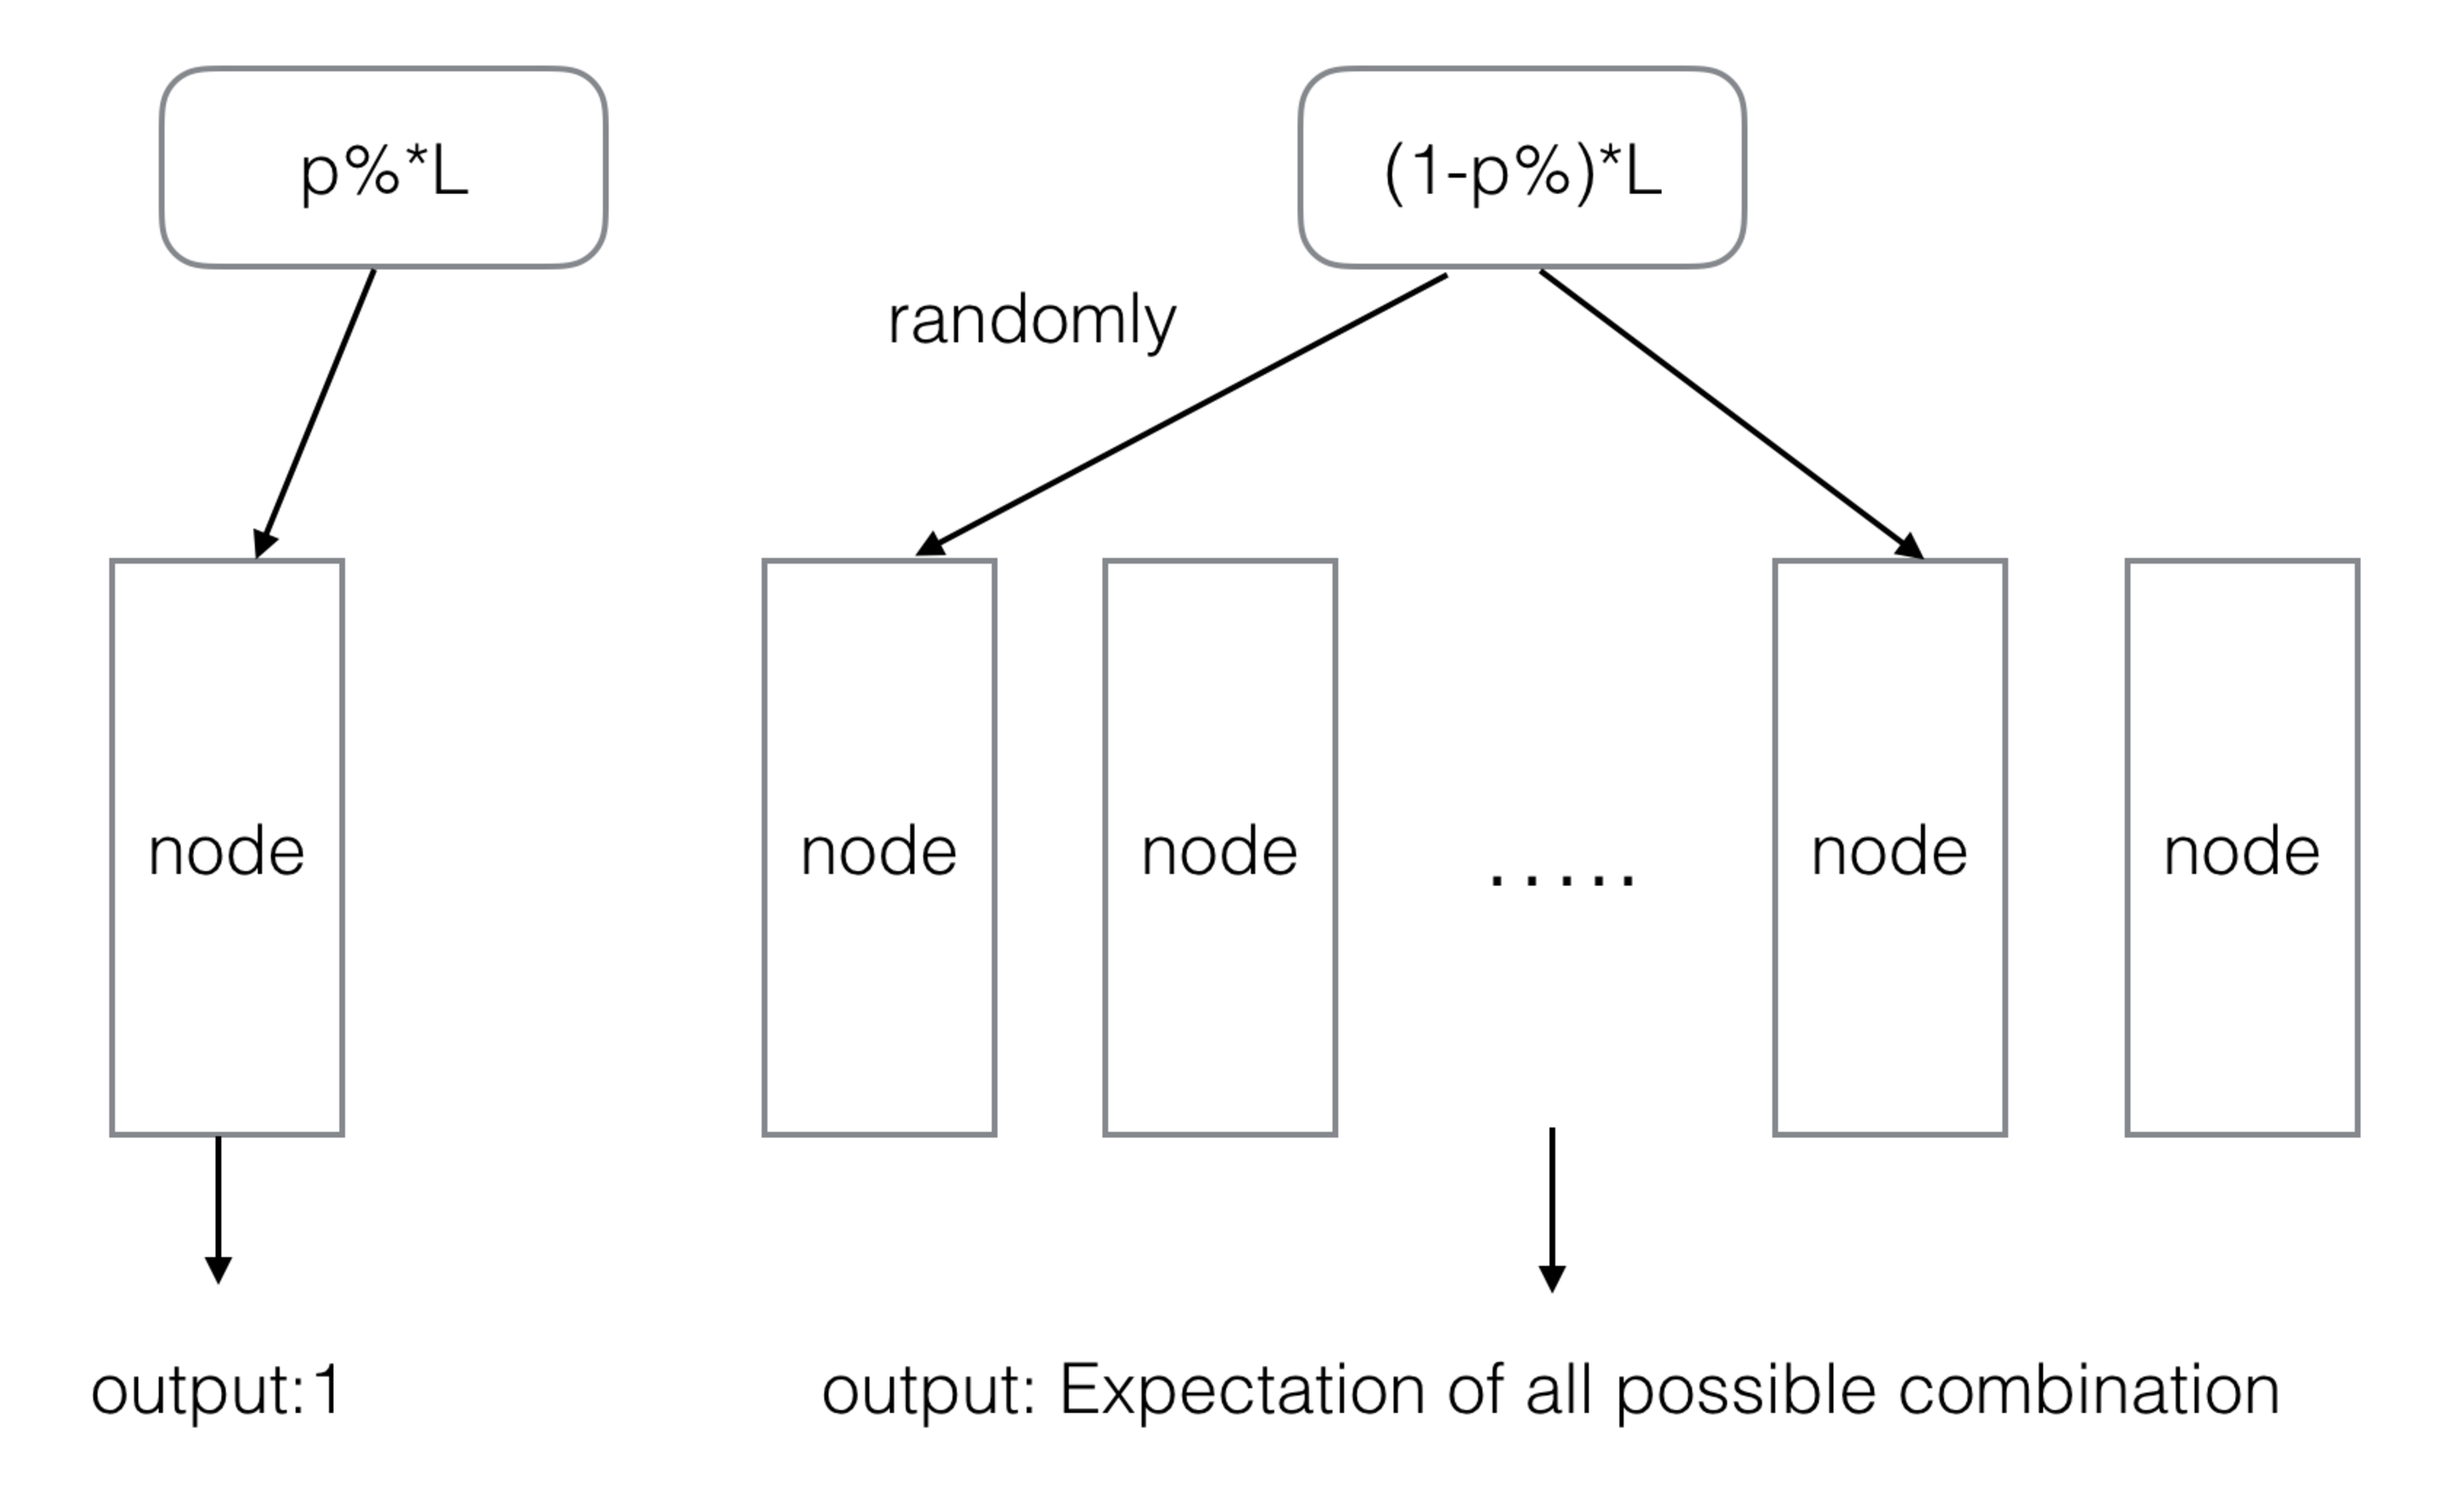
\includegraphics[scale=0.12]{fig5}
\caption{Expectation of combine ratio}
\label{fig:fig5}
\end{figure}
\subsection{Bucket Similarity and Key-Value Pairs Reduction}
The distance between each bucket is measured using Jaccard index. The similarity of two buckets is directly proportional to the number of shared pairs. By increasing the average bucket similarity within each node, the expected combine ratio is also increased, and therefore reducing the number of key-value pairs generated from the combiners.
\section{Experiment Evaluation}
In this section, we evaluate the performance of our proposed method MST+Spectral Clustering combiner. Two comparators used in our experiment are the hadoop default combiner and MST+ greedy combiner. For the hadoop default combiner. We just follow the hadoop defined combiner to implement it. For the MST + greedy combiner, we use MST to do the bucket allocation and greedy method to do the bucket selection.
\subsection{Experiment Setup}
\subsubsection{Datasets and evaluation metrics}
We use a real dataset from UC Irvine KDD repository. The Forest Covertype dataset are composed by 581,012 of 10-dimensional vectors of real numbers, each vector in the datasets represents a forest region in the Rock Mountain area.The evaluation metrics are showed in table 3.
We use two measures for the evaluation:combine ratio and execution time.The combine ratio is the data save after performing combine.The execution time represents the time taken to perform the combine.
\subsubsection{System Enviroment and Parameter Setting}
We conducted the Experiment on two Intel(R) Xeon(R) CPU E5-2620 v2 @ 2.10GHz dual processor server with 96GB memory. All all algorithm were implement using cython.
We set the number of hash functions \textbf{L} to 600 and number of buckets \textbf{B} to $2^{8}$, the replication factor of the bucket /textbf{R} is set to 5, the default number of node \textbf{N} is set to 12 and the default queryset size \textbf{Q} are set to 20000.Table 3 provides a summary of these parameter values we used in the experiments.
\begin{table} [h]
\centering
\caption{Default parameter}
\label{tab:table}
\begin{tabular}{|c|c|} \hline
Parameter & Value\\\hline
HashFuctionNumber & 600 \\\hline
BucketNumber & $2^{8}$\\\hline
Replication Factor & 5\\\hline
QSize & 20k\\\hline
PSize & 100k\\\hline
NodeNumber & 12\\\hline
\end{tabular}\\
\end{table}

\subsection{Experiment Result}
In this subsection, we report results from our experiments. A summary of results obtained by setting all parameters to the default values is shown in Table 4. Our method MST+Spectral Clustering improved the combine ratio to 50\%, the default combiner can reduce about 15\% of the data. That means our method can reduce 3.3 times of data than the default one and  1.13 times of data than the MST+greedy method. Our proposed method are also 1.53 times faster than the default method.

\begin{table} [h]
\centering
\caption{Default parameter Result}
\label{tab:table}
\begin{tabular}{|c|c|c|} \hline
Method & Combine Ratio & Execution Time(min)\\\hline
Default &15\% & 125  \\\hline
MST+Greedy & 44\% & 104 \\\hline
MST+Spectral Clustering & 50\% & 82 \\\hline
\end{tabular}\\
\end{table}

\subsubsection{Effect of L}
LSH is a Monto-Carlo method. So the number L is directly correlated to the accuracy of the method. In our experiment, we vary L from 200 to 800 hash functions. As shown in Figure 6, the combine ratio raises when we increase L, because it's more likely that the similar point pair have been hashed into the same bucket. The chance of allocate the similar bucket into the same node have also increased. Table 5 shows that in all the three methods the execution time increases as L increases. The increase in execution time is due to the increased  number of hash lookups we need to perform for each point pair.

\begin{figure}
\centering
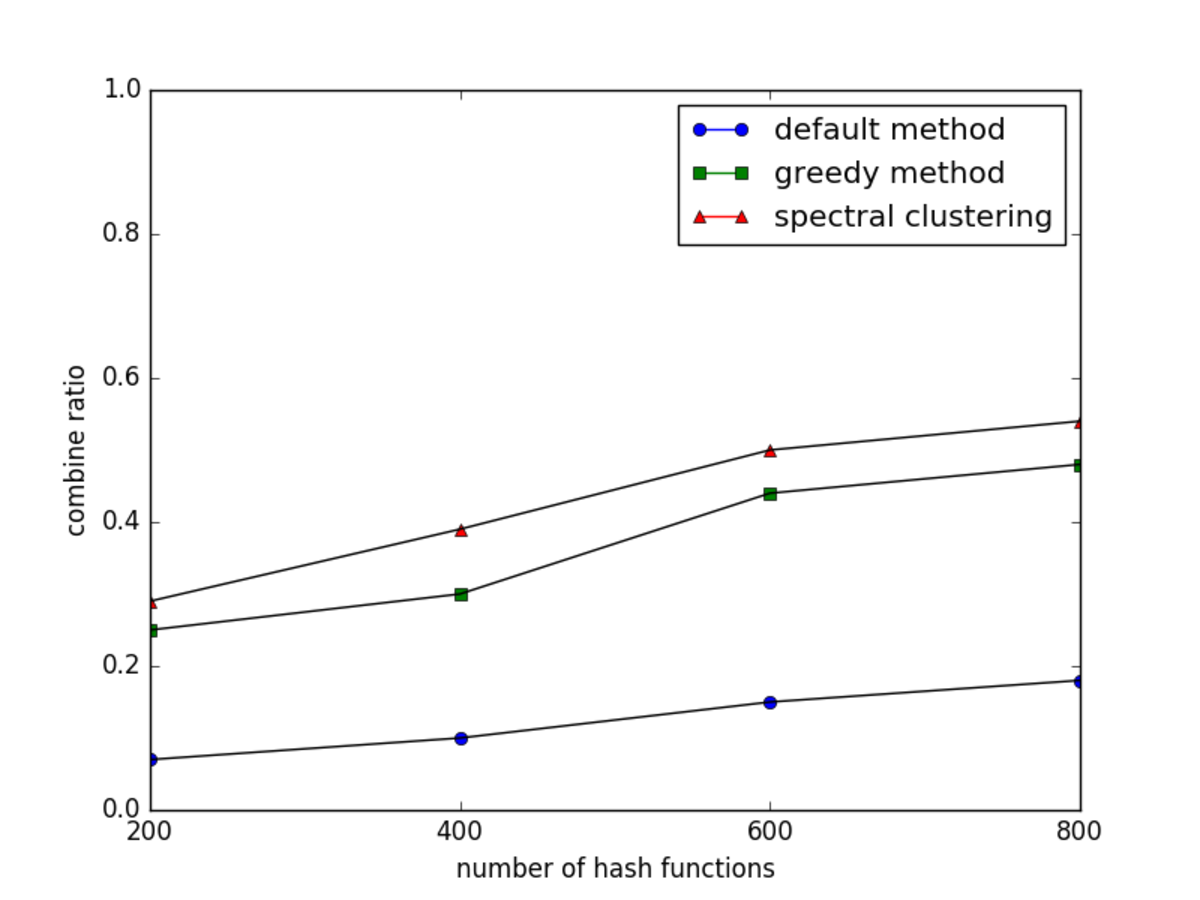
\includegraphics[scale=0.45]{FHashFunction}
\caption{Result for different number of Hash Functions}
\label{fig:HashFunction}
\end{figure}

\begin{table} [h]
\centering
\caption{execution time for different Number of Hash Functions}
\label{tab:table}
\begin{tabular}{|c|c|c|c|c|} \hline
Method & 200 & 400 & 600 & 800 \\\hline
Default & 40 & 67 & 125 & 167\\\hline
MST+Greedy & 33 & 50 & 104 & 131\\\hline
MST+Spectral Clustering & 26 & 39 & 82 & 98\\\hline
\end{tabular}\\
\end{table}

\subsubsection{Effect of R}
As part of setting up the cluster, you specify the number of copies of data that you want the cluster to maintain. The data is divided into buckets, and the cluster maintains multiple copies of each bucket. Each bucket copy is stored on a separate peer node. The number of data/bucket copies is called the cluster's replication factor. As shown in Figure 7, the combine ratio increase when we enlarge replication factor. Because after we enlarge the replication factor. The chance of clusters founded on one node became larger. Table 6 shows that when we increase the replication factor. The execution time also increased. Because when we increase R, the total block amount will increase. There are more buckets need to be process.

\begin{figure}
\centering
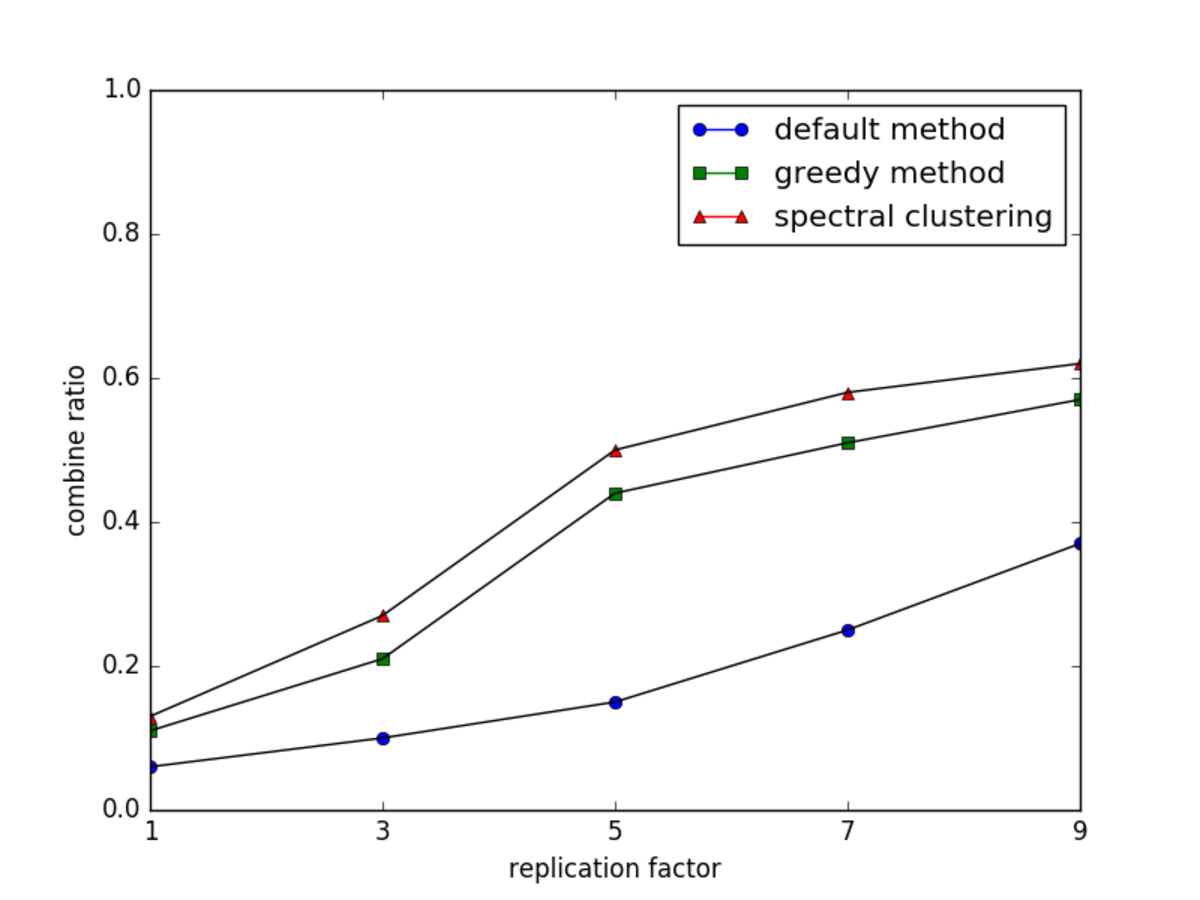
\includegraphics[scale=0.45]{FReplicationFactor}
\caption{Result for different Replication Factor}
\label{fig:ReplicationFactor}
\end{figure}

\begin{table} 
\centering
\caption{execution time for different replication factor}
\label{tab:table}
\begin{tabular}{|c|c|c|c|c|c|} \hline
Method & 1 & 3 & 5 & 7 & 9 \\\hline
Default & 103 & 117 & 125 & 142 & 153\\\hline
MST+Greedy & 77 & 86 & 104 & 112 & 121 \\\hline
MST+Spectral Clustering & 67 & 74 & 82 & 91 & 103 \\\hline
\end{tabular}\\
\end{table}

\subsubsection{Effect of B}
We study the effect of changing number of buckets B. We vary B from $2^{6}$ to $2^{10}$. Figure 9 shows the effect of B on combine ratio. Table 8 shows that the execution time increase as B increase.
\begin{figure}
\centering
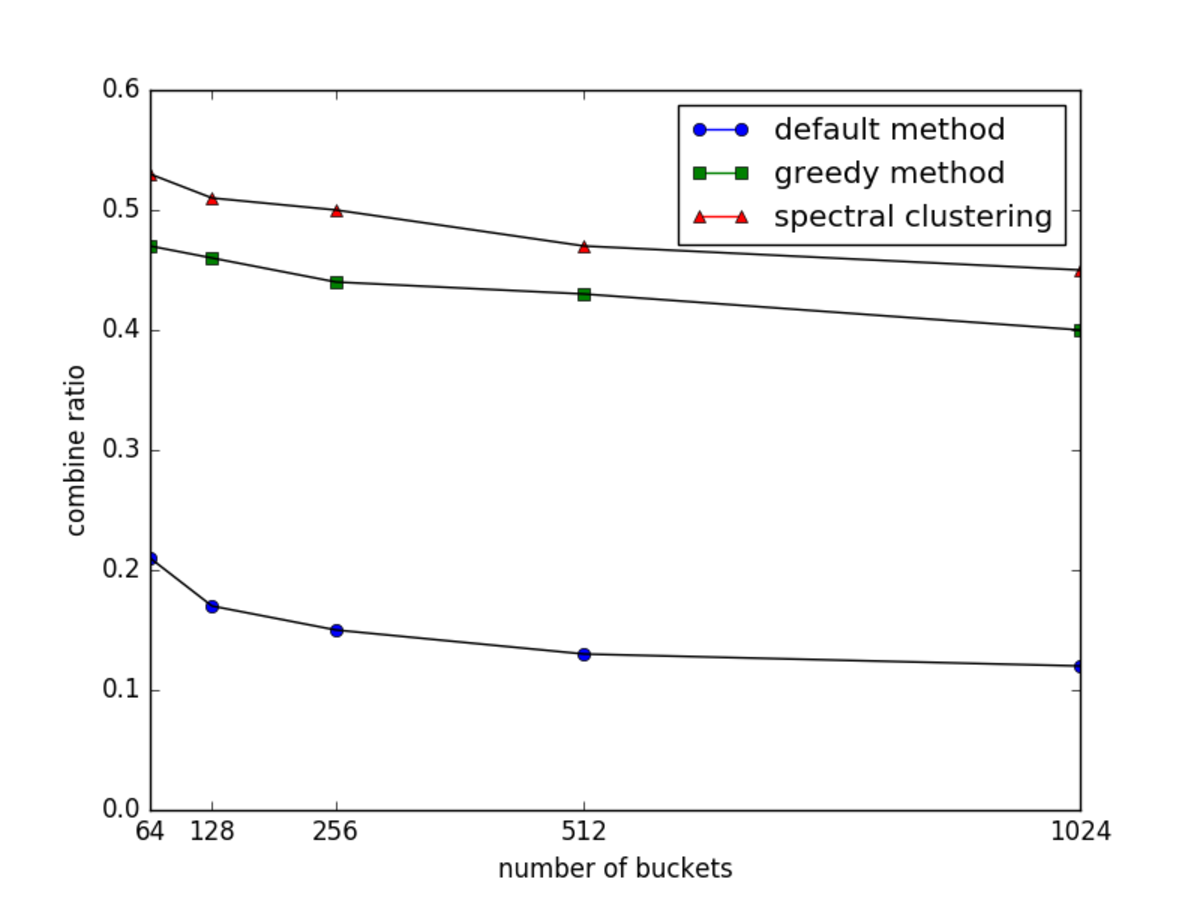
\includegraphics[scale=0.45]{FBucketNumber}
\caption{Result for different number of buckets}
\label{fig:BucketNumber}
\end{figure}

\begin{table} [h]
\centering
\caption{execution time for different Number of Bucket}
\label{tab:table}
\begin{tabular}{|c|c|c|c|c|c|} \hline
Method & $2^{6}$ & $2^{7}$ & $2^{8}$ & $2^{9}$ & $2^{10}$ \\\hline
Default & & & 125 & &\\\hline
MST+Greedy & & & 104 & & \\\hline
MST+Spectral Clustering & & & 82 & & \\\hline
\end{tabular}\\
\end{table}

\subsubsection{Effect of Q}
We also tested how our method scales when the number of query points Q increases. We set $\lvert Q \rvert$ from 10,000 to 50,000 query points. Figure 9 shows the effect of $\lvert Q \rvert$ on combine ratio. The combine ratio increases when we increase the number of query points Q. Table 8 shows that the execution time increase as $\lvert Q \rvert$ increase. This is because when Q increase the point pairs in the bucket also increase. That increases the Jaccard similarity computation time and the pairs need to be combine.
\begin{figure}
\centering
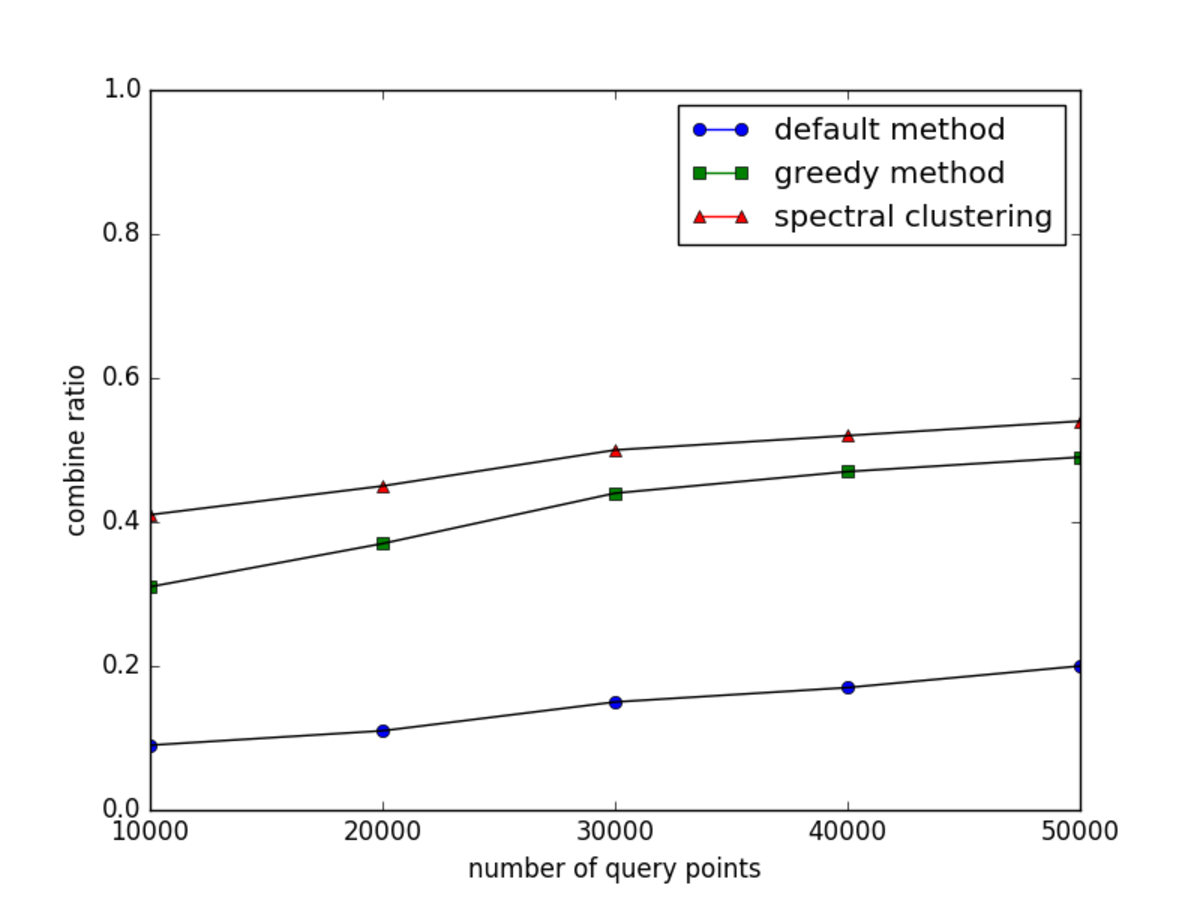
\includegraphics[scale=0.45]{FQueryPoints}
\caption{Result for different number of Query Points}
\label{fig:QueryPoints}
\end{figure}

\begin{table} [h]
\centering
\caption{execution time for different Number of QueryPoint}
\label{tab:table}
\begin{tabular}{|c|c|c|c|c|c|} \hline
Method & 10k & 20k & 30k & 40k & 50k \\\hline
Default & 72 & 125 & 221 & 285 & 364\\\hline
MST+Greedy & 51 & 104 & 147 & 213 & 248 \\\hline
MST+Spectral Clustering & 41 & 82 & 127 & 159 & 203\\\hline
\end{tabular}\\
\end{table}

\subsubsection{Effect of N}
We now study the effect of number of node N. Specifically, we vary N from 4 to 20. Figure 11 shows the effect of different number of nodes.As we can see the combine ratio are higher when we utilize smaller amount of node. Because if we use less nodes , the chance similar bucket allocate in the same node became higher. But it takes more time to execution the multiprocess ability are weaken than utilize a more nodes cluster as shown on Table 9.

\begin{figure}
\centering
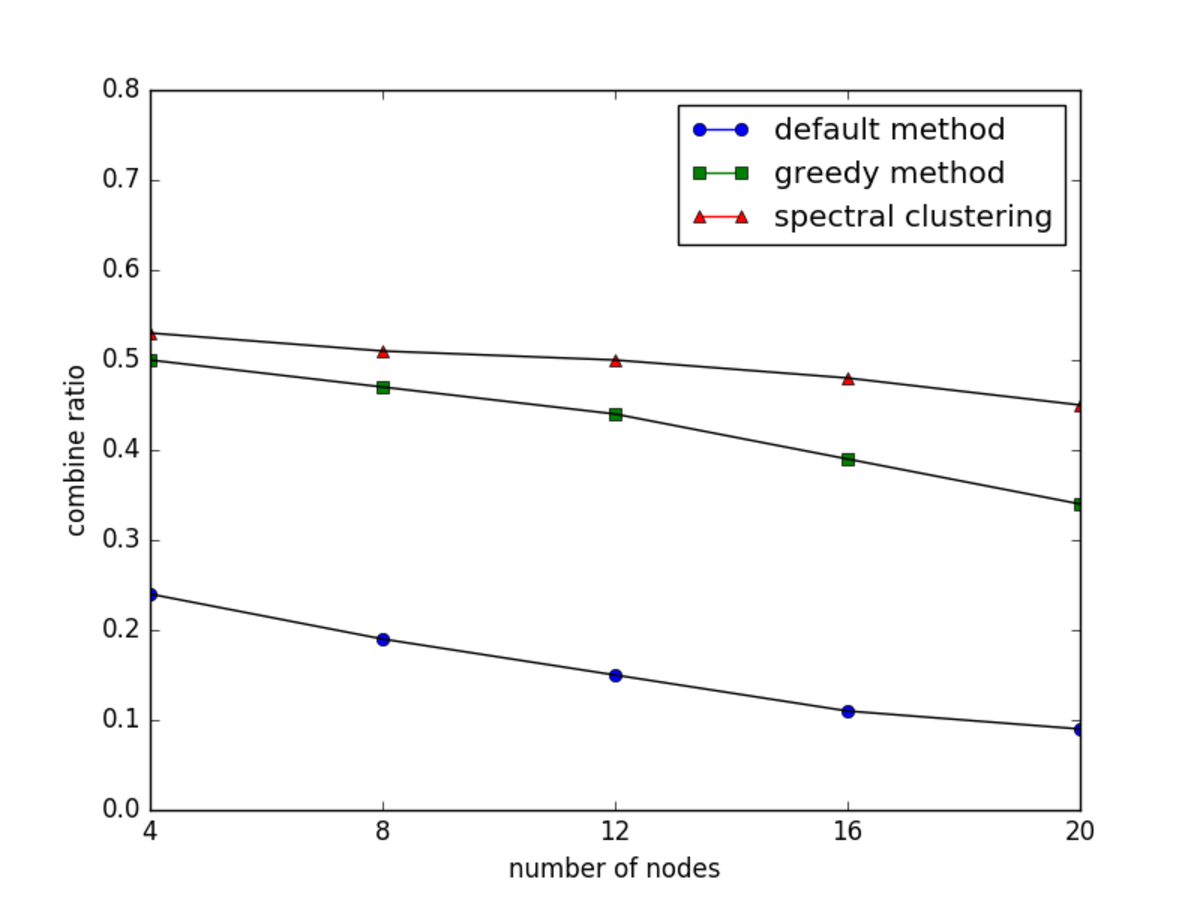
\includegraphics[scale=0.45]{FNodeNumber}
\caption{Result for different number of Nodes}
\label{fig:NodeNumber}
\end{figure}

\begin{table} [h]
\centering
\caption{execution time for different Number of Node}
\label{tab:table}
\begin{tabular}{|c|c|c|c|c|c|} \hline
Method & 4 & 8 & 12 & 16 & 20 \\\hline
Default & 362 & 187 & 125 & 84  & 78\\\hline
MST+Greedy & 294 & 154 & 104 & 74 & 62\\\hline
MST+Spectral Clustering & 237 & 121 & 82 & 60 & 51\\\hline
\end{tabular}\\
\end{table}

\subsubsection{Data Reduction Effect on Shuffler}
Since the data reduction will effect the shuffler's performance. So we conduct serval experiment to measure the benefit of our algorithm for the shuffler. We measure the data reduction size and the time saved in the shuffler stage. As shown on Figure 11 and Figure 12, The time saving on shuffle stage is no-lineal. It saves 1 time of the shuffle time while the data reduction is about 0.5 times.

\begin{figure}
\centering
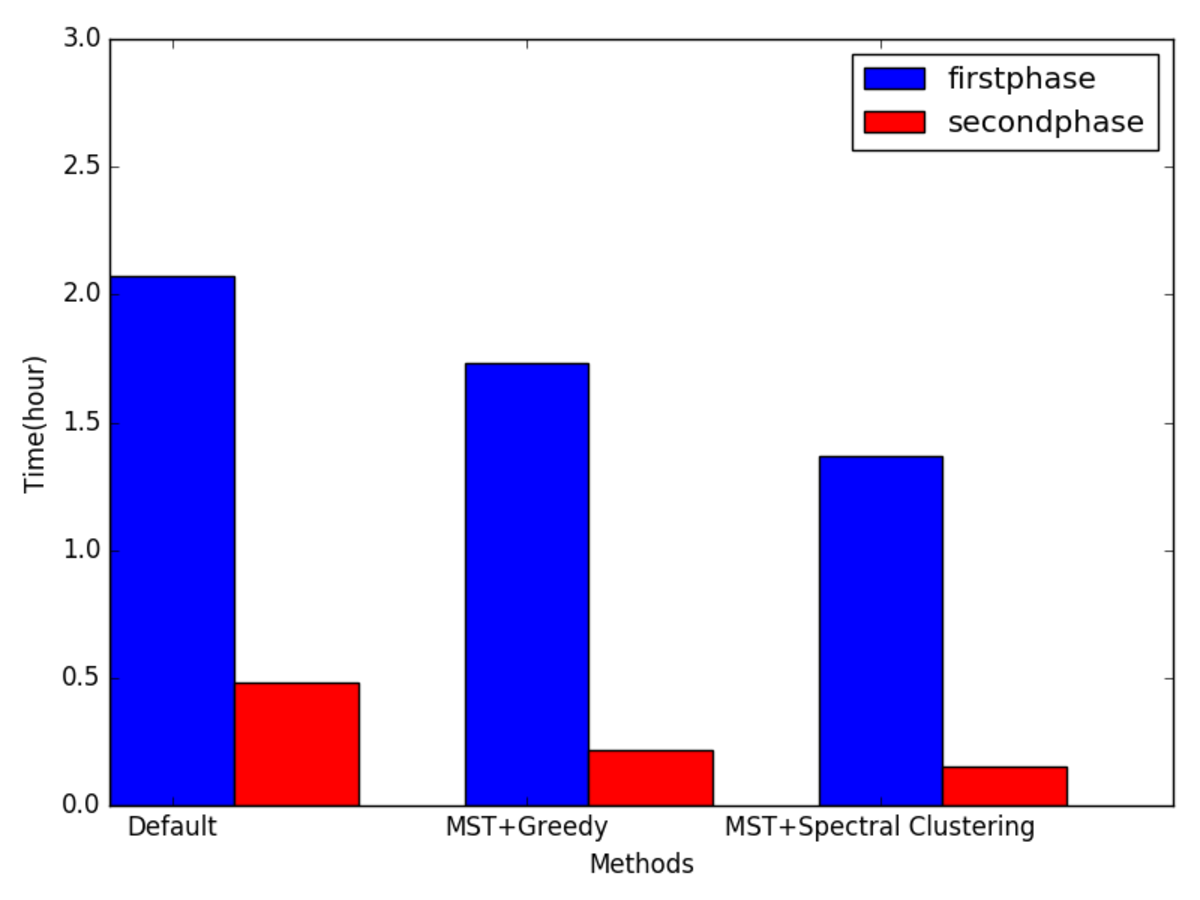
\includegraphics[scale=0.4]{FRunningTime}
\caption{Time Consuming for different Method}
\label{fig:RunningTime}
\end{figure}

\begin{figure}
\centering
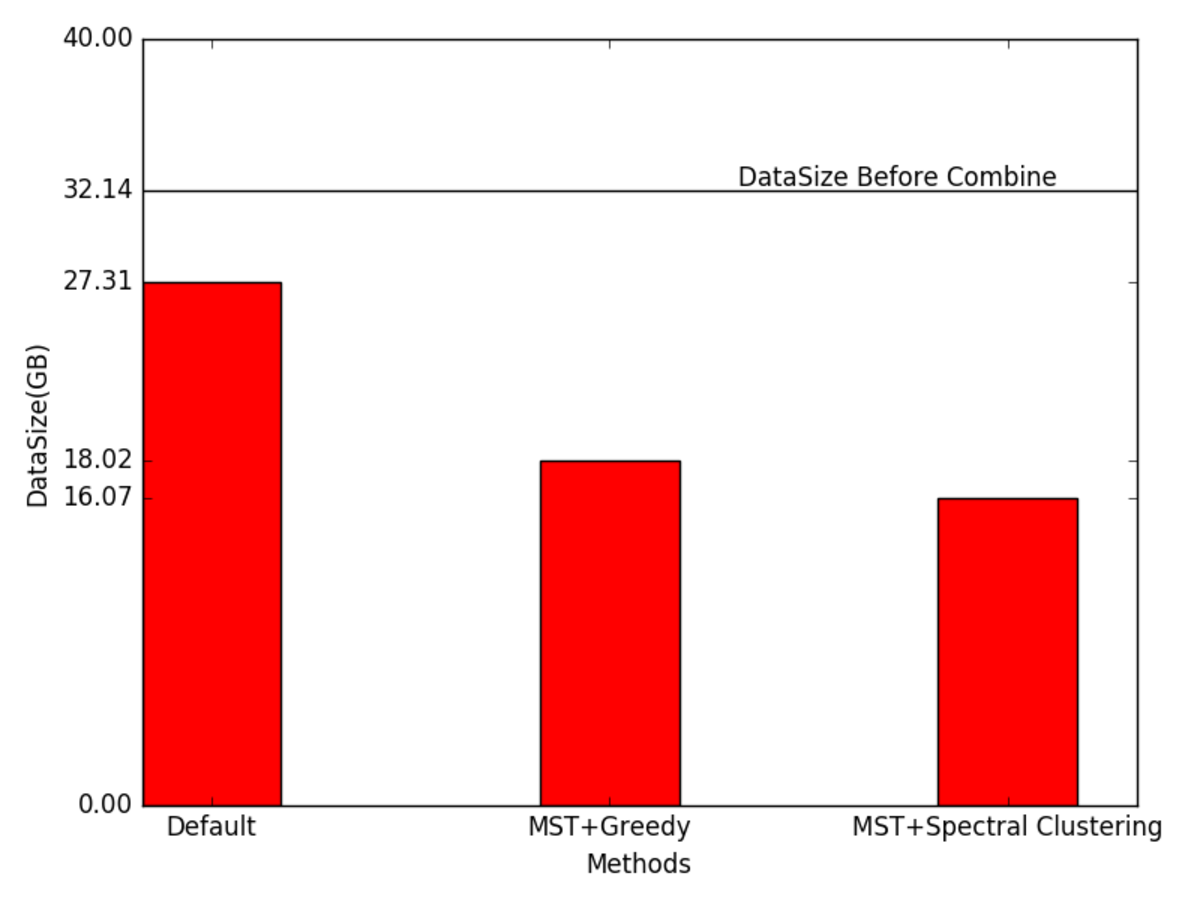
\includegraphics[scale=0.4]{FDataSizeReduction}
\caption{Data Reduction for different Method}
\label{fig:DataSizeReduction}
\end{figure}

\section{Conclusion}
In this paper, we propose two methods to speed up C2LSH-based similarity join on MapReduce by improving the utilization of MapReduce combiners. The first method is to apply MST-based partitioning on LSH buckets, and it improves the combine ratio by maximizing the bucket similarity in each partition. However, it has the limitation of not being able to maximize the combine ratio at run-time based on the query situation. The second method solves the limitation of the first method by introducing bucket replication to allow dynamic optimization of the combine ratio. Spectral clustering is used in the second method to allow run-time partition selection for maximizing the combine ratio. For cost analysis, we have derived the cost models for predicting the average combine ratio. Our experiment result shows that our method perform better than the other two method in both data reduction and time saving.\\
As future work, we plan to scale our algorithm to larger cluster and do some optimization make the algorithm performs even better.

%\end{document}  % This is where a 'short' article might terminate

% ensure same length columns on last page (might need two sub-sequent latex runs)
\balance

%ACKNOWLEDGMENTS are optional



% The following two commands are all you need in the
% initial runs of your .tex file to
% produce the bibliography for the citations in your paper.
\bibliographystyle{abbrv}
\bibliography{main}  % main.bib is the name of the Bibliography in this case
% You must have a proper ".bib" file
%  and remember to run:
% latex bibtex latex latex
% to resolve all references

\section{References}
[1] Apache Hadoop http://hadoop.apache.org/

[2] Apache Spark http://spark.apache.org/

[3] Approximate Nearest Neighbors: Towards Removing the Curse of Dimensionality 1998 Piotr Indyk, and Rajeev Motwani Proceedings of 30th Symposium on Theory of Computing, pages 604-613

[4] Approximate String Similarity Join using Hashing Techniques under Edit Distance Constraints 2014 Peisen Yuan, Haoyun Wang, Jianghua Che, Shougang Ren, Huanliang Xu, and Dechang Pi
Journal of Software, Volume 9, No 10, pages 2721-2731

[5] A Tutorial on Spectral Clustering 2007 Ulrike von Luxburg Statistics and Computing, Volume 17, Issue 4, pages 395-416

[6] Efficient Similarity Join for Time Sequences Using Locality Sensitive Hash and Mapreduce 2013 Dehua Chen, Liangliang Zheng, Meng Zhou, and Shoujian Yu Proceedings of 2013 International Conference on Cloud Computing and Big Data (CloudCom-Asia), pages 529-533


[7] Large-Scale Similarity Joins With Guarantees 2015 Rasmus Pagh Invited talk of 18th International Conference on Database Theory

[8] Locality-Sensitive Hashing Scheme Based on Dynamic Collision Counting 2012 Junhao Gan, Jianlin Feng, Qiong Fang, and Wilfred Ng Proceedings of the 2012 ACM SIGMOD International Conference on Management of Data, pages 541-552

[9] Locality-Sensitive Hashing Scheme Based on p-Stable Distributions 2004 Mayur Datar, Nicole Immorlica, Piotr Indyk, and Vahab S. Mirrokni Proceedings of the 20th Annual Symposium on Computational Geometry, pages 253-262

[10] MapReduce Based Personalized Locality Sensitive Hashing for Similarity Joins on Large Scale Data 2015 Jingjing Wang, and Chen Lin Computational Intelligence and Neuroscience, Volume 2015, page 13

[11] MapReduce: Simplified Data Processing on Large Clusters 2004 Jeffrey Dean, and Sanjay Ghemawat Proceedings of the 6th conference on Symposium on Opearting Systems Design \& Implementation, Volume 6, page 10

[12]Memcached http://memcached.org/

[13]The algorithms of Kruskal and Prim 2001 Thomas H. Cormen, Charles E. Leiserson, Ronald L. Rivest, and Clifford Stein Introduction to Algorithms, 2nd Ed., Section 23.2, pages 567-574

[14]Top-k Similarity Join in Heterogeneous Information Networks 2015 Yun Xiong, Yangyong Zhu, and Philip S. Yu Knowledge and Data Engineering, IEEE Transactions, Volume 27, Issue 6, pages 1710-1723

[15]A. Gionis, P. Indyk, and R. Motwani, ?Similarity search in high dimensions via hashing,in VLDB, 1999, pp. 518?529.

[16]R. Panigrahy, Entropy based nearest neighbor search in high dimensions in ACM-SIAM symposium on Discrete algorithm, 2006, pp. 1186? 1195.

[17]W. Dong, M. Charikar, and K. Li, ?Efficient k-nearest neighbor graph construction for generic similarity measures,? in WWW, 2011, pp. 577?586.
%APPENDIX is optional.
% ****************** APPENDIX **************************************
% Example of an appendix; typically would start on a new page
%pagebreak




\end{document}
